%
% vim:set expandtab tabstop=4 shiftwidth=4:
%


\section{Data Organization}
\label{section:DataOrg}

openBliSSART's data storage consists of a SQLite database \cite{SQLite} (in the
{\tt db} directory of the installation tree) in conjunction with an archive of
binary files (in the {\tt storage} directory). The database stores information
about the available objects (such as components generated by the NMF), their
features and class labels, while the object data itself is externalized to
binary files.

Generally\footnote{The separation process can also be run in a ``volatile'' mode
  that does not store anything. This is useful for example if the result of a
  NMF separation should be output as WAV files. See section
  \ref{section:septool} for details.}, when processing audio files, e.g. by FFT
and/or NMF, openBliSSART saves information about the separation process, such as
the name of the input file, the number of components, the STFT parameters
etc. in a respective \emph{process} entity. Furthermore, the computed objects
(such as NMF components) are saved as \emph{classification objects}. Each
classification object consists of one or more \emph{data descriptors} which
describe data like spectral vectors or phase matrices.

\paragraph{Classification Objects} openBliSSART currently creates and handles
the following types of classification objects:
\begin{center}
  \begin{tabular}{|p{.3\textwidth}|p{.6\textwidth}|}
    \hline
    NMD component & generated by applying STFT and NMD or NMF
    to an audio file \\
    Spectrogram & generated by applying STFT to an audio file \\
    \hline
  \end{tabular}
\end{center}

\paragraph{Data Descriptors} The following types of data descriptors are used:
\begin{center}
  \begin{tabular}{|p{.3\textwidth}|p{.6\textwidth}|}
    \hline
    Magnitude matrix & the magnitude spectrogram of an audio file \\
    Phase matrix & the phase spectrogram of an audio file \\
    Spectrum & a magnitude spectrum, generated by NMF or NMD from an audio file; a vector in case of NMF, or a matrix in case of NMD \\
    Gains & a gains vector, generated by NMF or NMD from an audio file \\
    \hline
  \end{tabular}
\end{center}
Note that it is perfectly valid for a data descriptor to occur in relation to
more than one classification object. For example, each classification object
generated by a NMF process contains a reference to the phase matrix of the
original signal so as to be able to re-synthesize wave files from one or more
components. The phase matrix, however, is stored only once.

Each data descriptor is associated with a separation process with a unique ID.
These IDs can for instance be found out by looking at the process listing in
the browser application, and are needed for component feature extraction
as well as data export.

\paragraph{Features, Responses and Labels} Data descriptors relate to
\emph{features} which are used during classification. A \emph{response} assigns
classification objects to \emph{labels}. Classification is done using features
from the data descriptors that make up the classification objects in the
response.\\

\noindent The browser (\ref{section:browser}) can be used to conveniently
explore the database structure.

\subsection{Database entities}

\label{subsection:DatabaseEntities}

A graphical overview over database entities and their relations
(entity-relationship diagram) is given by figure \ref{figure:ER}.

\begin{figure}
    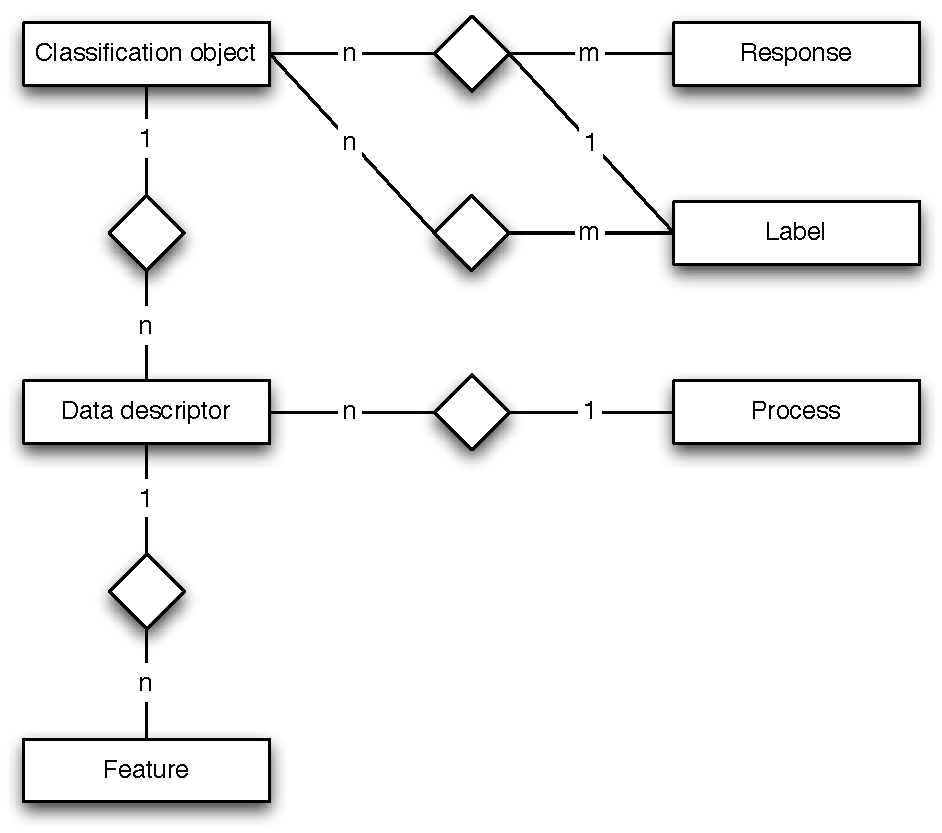
\includegraphics[width=\textwidth]{images/ERDiagram.pdf}
    \caption{%
        \label{figure:ER}
        Entity-relationship diagram of our database scheme
    }
\end{figure}


\paragraph{Processes}

A \emph{process} creates objects by processing an audio file. It has the
following attributes:
\begin{itemize}
    \item   Process ID
    \item   Name
    \item   Input file name
    \item   Sample frequency of the input file
    \item   Time at which the process was started
\end{itemize}
Furthermore, each process can have an arbitrary number of named parameters,
where the parameter value can be of any data type.


\paragraph{Data descriptors}

A \emph{data descriptor} contains information (``meta-data'') about a data
object, such as a vector or a matrix, which is stored as a file. The data
descriptor entity has the following attributes:
\begin{itemize}
    \item Data descriptor ID
    \item ID of the process that created the data object
    \item Type annotation, in our system one of ``Gains vector'', ``Spectral
      vector'' or ``Phase matrix''
    \item Index (in our NMF case, the component index for gains and spectral
      vectors, zero for phase matrices)
    \item Data availability flag. Functions that need the binary data ignore
      data descriptors whose data availability flag is false. This makes it
      possible to migrate the database to another computer without copying all
      the externalized binary data, in a consistent way.
\end{itemize}
Besides the data descriptor ID, the triple (process ID, type annotation, index)
uniquely identifies a data descriptor.


\paragraph{Classification objects}

A \emph{classification object} consists of several data objects described by
data descriptors. For example, in our application, we want to classify
components generated by a NMF process, which consist of a gains vector and a
spectral vector.

A classification object has a unique ID and a type annotation (in our case, the
only possible annotation is ``NMF component''); and furthermore, a list of IDs
of data descriptors that make up the classification object.

Finally, for each classification object a preselection of possible class labels
is stored. For example, a drum component could be labelled with ``Drum'' or,
more specifically, with ``Snare drum''.

Classification objects are subject to the following constraints:
\begin{itemize}
    \item   All data descriptors that make up the object must be created by the
            same process.
    \item   Every type of data descriptor (determined by the ``type
            annotation'' attribute) may occur at most once.
\end{itemize}


\paragraph{Features}

A \emph{feature} is a named value assigned to a data object, for example, a
cepstral coefficient of a spectral vector. Thus, the following attributes are
required:
\begin{itemize}
    \item   ID of the data descriptor describing the data object
    \item   Feature name (e.g. ``MFCC'')
    \item   Feature parameter (e.g. the coefficient index in the MFCC case)
    \item   Feature value
\end{itemize}
Every feature of a data object can be uniquely identified by feature name and
parameter.


\paragraph{Labels}

A \emph{label} is a textual class label that can be assigned to classification
objects. In our case, we could define the labels ``Drum'', ``Harmonic'' or more
specific labels like ``Guitar'' or ``Snare drum''.


\paragraph{Responses}

A \emph{response} is an assignment of classification objects to labels.
Additionally, every response has a response ID, a name (e.g. ``Drum vs.
Harmonic'') and a textual description.


\subsection{Storage of binary files}
\label{subsec:FileFormats}

Binary files corresponding to data objects, \ie vectors and matrices, are
stored in a directory layout such that the file name can be uniquely determined
by the attributes of the corresponding data descriptor.

All multi-byte values are saved in little-endian order.

Our binary file format for vectors consists of the following elements:
\begin{itemize}
    \item Orientation header (0 = row vector, 1 = column vector) (as 32 bit {\tt unsigned int})
    \item Vector dimension (32 bit {\tt unsigned int})
    \item Array of components (64 bit {\tt double})
\end{itemize}

Our binary file format for matrices consists of the following elements:
\begin{itemize}
    \item Matrix header = 2 (as 32 bit {\tt unsigned int})
    \item Number of rows (32 bit {\tt unsigned int})
    \item Number of columns (32 bit {\tt unsigned int})
    \item Array of matrix entries (64 bit {\tt double}) in column-major order,
      i.e. entry $a_{i,j}$ of a matrix with $m$ rows is stored at position $j *
      m + i$
\end{itemize}



\section{Source separation by NMF}


Non-Negative Matrix Factorization (NMF) is an algorithm originally proposed for
image decomposition \cite{LeeSeung1999}. As a method of information reduction,
its most promiment feature is the usage of non-negativity constraints: unlike
other methods such as Principal Components Analysis, it achieves a parts-based
representation where only additive -- never subtractive -- combinations of the
Given a matrix $\mat{V} \in \setR_{+}^{m \times n}$ and a constant $r \in \setN$,
non-negative matrix factorization (NMF) computes two matrices $\mat{W} \in \setR_{+}^{m
\times r}$ and $\mat{H} \in \setR_{+}^{r \times n}$, such that
\begin{equation}
    \label{math:BasicNMF}
    \mat{V} \approx \mat{WH}
\end{equation}

openBliSSART applies NMF in the frequency domain, by factorizing magnitude spectrogram matrices obtained by short-time Fourier transformation (STFT).
Thereby the signal is split into overlapping frames of constant size. In speech processing, it is common to use a frame size of 25\,ms and an overlap of 60\,\%, corresponding to a \emph{frame rate} of 10\,ms. Each frame is multiplied by a window function and transformed to the
frequency domain using Discrete Fourier Transformation (DFT), with transformation
size equal to the number of samples in each frame. 

First, openBliSSART provides the Hamming function for windowing

\begin{equation}
    h(k) = 0.54 - 0.46 \cos\left(\frac{2\pi k}{T-1} \right)
\end{equation}

\noindent where $T$ is the frame size and $k \in \{0, \dots, T\}$.

Other window functions are the Hann(ing) function:

\begin{equation}
    h(k) = 0.5 - 0.5 \cos\left(\frac{2\pi k}{T-1} \right)
\end{equation}

and its square root, which can be used for reducing artefacts resulting from
the transformation.

Only the magnitudes of the DFT coefficients are retained, and the frame spectra
are put in the columns of a matrix. Denoting the number of frames by $n$ and
the frame size by $T$, and considering the symmetry of the coefficients, this
yields a $\left( \lfloor T/2 \rfloor +1 \right) \times n$ real matrix. 

The crucial idea behind NMF-based blind source separation is to assume a
\emph{linear signal model}. Note that Eq. \ref{math:BasicNMF} can be written as
follows (the subscripts $:,t$ and $:,j$ denotes the $t^{\textrm{th}}$ and
$j^{\textrm{th}}$ matrix columns, respectively):

\begin{equation}
    \label{math:LinSigMod}
    \mat{V}_{:,t} \approx \sum\limits_{j=1}^r \mat{H}_{j,t} \mat{W}_{:,j}, \quad 1 \leq t \leq n
\end{equation}

Thus, if $\mat{V}$ is the magnitude spectrogram of a signal (with short-time spectra
in columns), the factorization from Eq. \ref{math:BasicNMF} represents each short-time spectrum
$\mat{V}_{:,t}$ as a linear combination of spectral basis vectors
$\mat{W}_{:,j}$ with non-negative coefficients
$\mat{H}_{j,t}$ ($1 \leq j \leq r$). 


When there is no prior knowledge about the number of spectra that can describe
the source signal, the number of components $r$ has to be chosen empirically,
depending on the application.

\subsection{Basic NMF Algorithms}
\label{section:NMFAlg}

A factorization according to Eq. \ref{math:BasicNMF} is usually achieved by
iterative minimization of a cost function $c(\mat{W},\mat{H})$:
\begin{equation}
    \label{math:minimi}
    (\mat{W},\mat{H}) = \argmin\limits_{\mat{W},\mat{H}} c(\mat{W},\mat{H}) 
\end{equation}

In fact, many variants of NMF only differ by their choice of a particular cost
function.  The core of these functions is a measurement of the reconstruction
error between the original matrix and the product of the NMF factors.  Thus, a
basic cost function is the squared Euclidean distance between $\mat{V}$ and
$\mat{WH}$:

\begin{equation}
    \label{math:eudist}
    c_e(\mat{W},\mat{H}) = 
    ||\mat{V}-\mat{WH}||_F = 
    \sum_{i=1}^n \sum_{j=1}^m (\mat{V}-\mat{WH})_{i,j}^2 ,
\end{equation}
where $||.||_F$ denotes the Frobenius norm.  

Another cost function consists of a modified version of Kullback-Leibler (KL) divergence:

\begin{equation}
    \label{math:kldiv}
    c_d(\mat{W},\mat{H}) = \sum\limits_{i=1}^m \sum\limits_{t=1}^n
    \left( \mat{V}_{i,t} \log\frac{\mat{V}_{i,t}}{(\mat{W}\mat{H})_{i,t}} - 
    (\mat{V} - \mat{W}\mat{H})_{i,t} \right)
\end{equation}

For minimization of either cost function, openBliSSART implements the two algorithms by
Lee and Seung \cite{LeeSeung2001}, which iteratively modify $\mat{W}$ and
$\mat{H}$ using `multiplicative update' rules. It can be shown that $c_e$ is
non-increasing under the update rules

\begin{equation}
    \label{math:EDHUpdateRule}
    \mat{H}_{j,t} \leftarrow \mat{H}_{j,t} \,
    \frac{( \mat{W}^T \mat{V} )_{j,t}}
         {( (\mat{W}^T \mat{W})\mat{H} )_{j,t}}
    \qquad
    j = 1, \dots, r; t = 1, \dots, n
\end{equation}

\begin{equation}
    \label{math:EDWUpdateRule}
    \mat{W}_{i,j} \leftarrow \mat{W}_{i,j} \,
    \frac{( \mat{VH}^T )_{i,j}}
         {( \mat{W} (\mat{H}\mat{H}^T) )_{i,j}}
    \qquad
     i = 1, \dots, m; j = 1, \dots, r
\end{equation}

\noindent and that $c_d$ is non-increasing under the update rules

\begin{equation}
    \label{math:KLHUpdateRule}
    \mat{H}_{j,t} \leftarrow \mat{H}_{j,t} \,
    \frac{(\mat{W}^T (\mat{V} ./ \mat{W}\mat{H}))_{j,t}}
         {(\mat{W}^T \mat{1})_{j,t}}
    \qquad
    j = 1, \dots, r; t = 1, \dots, n
\end{equation}

\begin{equation}
    \label{math:KLWUpdateRule}
    \mat{W}_{i,j} \leftarrow \mat{W}_{i,j} \,
    \frac{((\mat{V} ./ (\mat{WH})) \mat{H}^T)_{i,j}}
         {(\mat{1H}^T)_{i,j}}
    \qquad
     i = 1, \dots, m; j = 1, \dots, r .
\end{equation}
where $\mat{1}$ is an all-unity matrix and $./$ indicates elementwise division.
The above matrix formulation has been shown to yield better performance than
the scalar product formulations in \cite{LeeSeung2001} when using fast
implementations of matrix multiplication, as openBliSSART does.

Thereby the denominators are floored to a very small positive constant (such as
$10^{-10}$) to avoid divisions by zero. Note that these rules are applied
alternatingly, with each $\mat{W}$ update using the new value of $\mat{H}$ that
was calculated in the previous $\mat{H}$ update and vice versa. Note that the
order of calculation, indicated by the parentheses in
Eq.~\ref{math:EDHUpdateRule} and Eq.~\ref{math:EDWUpdateRule} can have a great
effect on performance due to the different matrix dimensions.


\subsection{Initialization and Termination}

For conventional, i.\,e.\ unsupervised NMF, $\mat{W}$ and $\mat{H}$ can be initialized with the absolute values of random numbers drawn from a
Gaussian distribution with $\mu = 0$ and $\sigma = 1$, or from a uniform distribution on the interval $]0,1]$. 

openBliSSART uses the following stopping criterion for NMF:

\begin{equation}
    \label{math:stopping}
    \frac{||\mat{W}^{q+1}\mat{H}^{q+1} - \mat{W}^{q}\mat{H}^{q}||_F}
         {||\mat{W}^{q}\mat{H}^{q}||_F}
    < \zeta ,
\end{equation}

\noindent with $\mat{W}^q$ and $\mat{H}^q$ denoting the values of $\mat{W}$ and
$\mat{H}$ at iteration $q$, respectively, and $\zeta$ being a small constant.
However, evaluation of the criterion \ref{math:stopping} is costly, as the
matrix product $\mat{WH}$ has to be computed, and the previous values of
$\mat{W}$ and $\mat{H}$ (or the previous value of their product) have to be
stored. Thus, to reduce computational cost, it is preferred to perform a \emph{fixed
number} of iterations. Experience shows that 100--200 iterations ensure a small
reconstruction error which is not significantly reduced by further iterations.


\subsection{Supervised Component Classification}

\label{sec:nmfbss}

In scenarios like speaker separation or drum accompaniment reduction, sources
(speakers, drums) can often not be modelled by a single spectrum. NMF-based
approaches in this area thus have to use a number $r$ of components which is
larger than the number of sources. Consequently, an assignment of the
components to sources has to be made.

For the following discussion, we formally define the $j^{\textrm{th}}$
component of the signal to be the pair $\left(\bv{w}_j, \bv{h}_j\right)$ of a
spectrum $\bv{w}_j := \mat{W}_{:,j}$ along with its time-varying gains
$\bv{h}_j := \mat{H}_{j,:}$ (the subscript $j,:$ denotes the $j^{\textrm{th}}$
matrix row).

openBliSSART uses the following approach to decide which components belong to which source. First, a Support Vector Machine (SVM) classifier is trained from the features in a {\em response variable} according to Section \ref{section:DataOrg}. After classification, a magnitude
spectrogram $\mat{V}_{s_i}$ for each source $s_i$ can be computed: let

\begin{equation}
    \label{math:Jsi}
    J_{s_i} = \left\{ j: \left(\bv{w}_j, \bv{h}_j\right) 
                         \mbox{assigned to } s_i \right\}
\end{equation}

\noindent be the set of indices of components assigned to source $s_i$. Then,

\begin{equation}
    \label{math:Vharm}
    \mat{V}_{s_i} = \sum\limits_{j \in J_{s_i}} \bv{w}_j \bv{h}_j .
\end{equation}

$\mat{V}_{s_i}$ is transferred back to the time domain using a column-wise
inverse IDFT, using the phase matrix from the original signal. Finally, time
signals for each source are obtained by adding up the time frames respecting
their overlap. Multiplication of the time frames with the square root of the Hann function can
reduce the artifacts resulting from the transformation \cite{Virtanen2005}.


\subsection{Source Separation by Supervised NMF}

\label{sec:nmfsss}

Supervised NMF means that Thereby $\mat{W}$ is
set to a predefined matrix where each column contains a spectrum corresponding
to one of the sources. For example, in speaker separation these spectra can be
computed from phonemes uttered by a certain speaker \cite{Schmidt2006}. 

Then $\mat{W}$ is kept constant throughout
the iteration whereas $\mat{H}$ is initialized randomly and updated
iteratively. Time
signals for each source can be obtained using the procedure which was mentioned
above, setting $J_{s_i}$ (Eq.~\ref{math:Jsi}) to the indices of columns of
$\mat{W}$ that were initialized with spectra from source $s_i$. This paradigm
has led to notable results in speech denoising \cite{Wilson2008_1,Wilson2008_2}
and speaker spearation \cite{Schmidt2006,Grady2007}. 


\subsection{Sparse NMF}
\label{sec:sparseness}

The aforementioned cost functions measure the reconstruction error $c_r$.
However, for overcomplete bases (\ie $r > m,n$) sparse NMF \cite{Hoyer2002,Hoyer2004,Eggert2004,Schmidt2006,Virtanen2007} can be valuable, whereby a term is added that increases the value of the cost function for each non-zero entry in
$\mat{H}$, hence `dense' matrices are penalized. The resulting cost function
$c(\mat{W},\mat{H}$) is

\begin{equation}
    \label{math:costsparseness}
    c(\mat{W},\mat{H}) = c_r(\mat{W},\mat{H}) + \lambda c_s(\mat{H})
\end{equation}

\noindent where $c_r(\mat{W},\mat{H})$ can -- for example -- be set to squared
Euclidean distance (Eq.~\ref{math:eudist}) or modified KL divergence
(Eq.~\ref{math:kldiv}).

First, openBliSSART supports a straightforward approach introduced by \cite{Virtanen2007}:

\begin{equation}
    \label{math:sparseness} 
    c_s(\mat{H}) = \sum\limits_{j=1}^r \frac{1}{\sigma_j} \sum\limits_{t=1}^n \mat{H}_{j,t}
\end{equation}

To prevent the scaling from affecting the value of the cost
function, it normalizes the activations of each component $j$, \eg
by their standard deviation estimates $\sigma_j$ \cite{Virtanen2007}. The multiplicative update rules for $\mat{H}$ minimizing the cost function \ref{math:costsparseness} are derived as follows. 

The gradient of the cost function is written as a subtraction $\nabla c(\mat{W},\mat{H}) = \nabla c^+ (\mat{W},\mat{H}) - \nabla c^- (\mat{W},\mat{H})$ of element-wise nonnegative terms $\nabla c^+(\mat{W},\mat{H}) = \nabla c_r^+(\mat{W},\mat{H}) + \lambda \nabla c_s^+(\mat{H})$ and $\nabla c^-(\mat{W},\mat{H}) = \nabla c_r^-(\mat{W},\mat{H}) + \lambda \nabla c_s^-(\mat{H})$.
For Euclidean distance, we have 
\begin{equation}
\nabla c_r^+(\mat{W},\mat{H}) = \mat{W}^T\mat{WH}
\end{equation}
and
\begin{equation}
\nabla c_r^-(\mat{W},\mat{H}) = \mat{W}^T\mat{V}
\end{equation}

For KL divergence, we have:
\begin{equation}
\nabla c_r^+(\mat{W},\mat{H}) = \mat{W}^T\mat{1}
\end{equation}
and
\begin{equation}
\nabla c_r^-(\mat{W},\mat{H}) = \mat{W}^T (\mat{V} ./. (\mat{WH}))
\end{equation}

For the sparseness term, we have:

\begin{equation}
[\nabla c_s^+(\mat{H})]_{j,t} = \frac{1 / \sqrt{n}}{\sqrt{\sum_{k=1}^n \mat{H}_{j,k}^2}}
\end{equation}
and
\begin{equation}
[\nabla c_s^-(\mat{H})]_{j,t} = \mat{H}_{j,t} \frac{\sqrt{n}\sum_{k=1}^n \mat{H}_{j,k}}{(\sum_{k=1}^n \mat{H}_{j,k}^2)^{3/2}}
\end{equation}

The final multiplicative update rule is:

\begin{equation}
\mat{H}_{j,t} \leftarrow \mat{H}_{j,t}\frac{\nabla_c^-(\mat{W},\mat{H})}{\nabla_c^+(\mat{W},\mat{H})}
\end{equation}


As a second approach to sparse NMF, openBliSSART implements the algorithm from
\cite{Eggert2004} which is based on a cost function resembling Euclidean
distance with a column-wise normalized $\mat{W}$ matrix. openBliSSART
reformulates the multiplicative update rules for enhanced performance:
\begin{equation}
\mat{H}_{j,t} \leftarrow \mat{H}_{j,t} 
    \frac{(\mat{W}^T \mat{V})_{j,t}}
         {((\mat{W}^T\mat{W})\mat{H})_{j,t} + \lambda}
\end{equation}
where $\lambda$ is the sparseness weight, and
\begin{equation}
\mat{W}_{i,j} \leftarrow \mat{W}_{i,j} 
    \frac{(\mat{VH}^T)_{i,j} + ((\mat{HH}^T)(\mat{W}^T\mat{W}))_{j,j} \hat{\mat{W}}_{i,j}}
         {(\mat{W}(\mat{HH}^T))_{i,j} + (\mat{HV}^T\mat{W})_{j,j} \hat{\mat{W}}_{i,j}}
\end{equation}
where $\hat{\mat{W}}$ is the column-wise normalized matrix $\mat{W}$ (Euclidean
norm).


\subsection{Convolutive NMF}

\label{sec:NMD}

\emph{Convolutive} variants of NMF 
consider spectra that evolve over time. In other words, the acoustic events
that build the signal are no longer instantaneous, but rather sequences of
observations. In speech processing, these sequences can correspond to phonemes
\cite{Smaragdis2007} or even whole words \cite{Smaragdis2004}. 

First, openBliSSART supports Non-Negative Matrix Deconvolution, which is based
on a convolutive signal model:

\begin{equation}
    \label{math:NMDFact}
    \mat{V} \approx \mat{\Lambda} = \sum\limits_{p=0}^{P-1} 
                                    \mat{W}(p) \overset{\rightarrow p}{\mat{H}}
\end{equation}

\noindent where $\mat{W}(p), p \in \{0,\dots,P-1\}$ is a set of $P$ matrices and
$\overset{\rightarrow p}{(\cdot)}$ is a matrix operator that shifts the
columns of its argument by $p$ spots to the right, filling the leftmost $p$
columns with zeros. Analogously to Eq.~\ref{math:LinSigMod}, this equation can
be rewritten as

\begin{equation}
    \label{math:ConvSigMod}
    \mat{V}_{:,t} \approx \sum\limits_{j=1}^r \sum\limits_{p=0}^{\min\{P-1,t\}}
    \mat{H}_{j,t-p} \mat{W}(p)_{:,j}, \quad 1 \leq t \leq n
\end{equation}

\noindent where again $r$ is the number of components and $n$ is the number of
columns of $\mat{V}, n \geq P$. (Note that the inner sum now resembles a
convolution.)

It is straightforward to extend the cost functions $c_e$ (Euclidean distance,
Eq.~\ref{math:eudist}) and $c_d$ (modified KL divergence, Eq.~\ref{math:kldiv})
to the convolutive signal model:

\begin{eqnarray}
    \label{math:eudistNMD}
    c_e' &=& ||\mat{V}-\mat{\Lambda}||_F = \sum\limits_{i=1}^n \sum\limits_{j=1}^m (\mat{V}-\mat{\Lambda})_{i,j}^2\\
    \label{math:kldivNMD}
    c_d' &=& \sum\limits_{i=1}^m \sum\limits_{t=1}^n
    \left( \mat{V}_{i,t} \log\frac{\mat{V}_{i,t}}{\mat{\Lambda}_{i,t}} - 
    (\mat{V} - \mat{\Lambda})_{i,t} \right)
\end{eqnarray}

A multiplicative update algorithm can be derived for either cost function
\cite{Smaragdis2004,WangNMD2009}. Note that there are now $P+1$ updates in each
iteration: one for each matrix $\mat{W}(p), p = 0, \dots, P-1$ and one for
$\mat{H}$. In detail, the update rules for minimization of $c_e'$
(Eq.~\ref{math:eudistNMD}) are given by

\begin{equation}
    \label{math:EDWUpdateRuleNMD}
    \mat{W}(p)_{i,j} \leftarrow \mat{W}(p)_{i,j} \,
    \frac{( \mat{V}(\overset{p\rightarrow}{\mat{H}})^T )_{i,j}}
         {( \mat{\Lambda}(\overset{p\rightarrow}{\mat{H}})^T )_{i,j}}
    \qquad
     i = 1, \dots, m; j = 1, \dots, r
\end{equation}

\begin{equation}
    \label{math:EDHUpdateRuleNMD}
    \mat{H}_{j,t} \leftarrow \mat{H}_{j,t} \, \frac{1}{P} \sum\limits_{p=0}^{P-1} 
    \frac{( \mat{W}(p)^T \overset{\leftarrow p}{\mat{V}} )_{j,t}}
         {( \mat{W}(p)^T \overset{\leftarrow p}{\mat{\Lambda}} )_{j,t}}
    \qquad
    j = 1, \dots, r; t = 1, \dots, n
\end{equation}

\noindent while $c_d'$ (Eq.~\ref{math:kldivNMD}) is minimized by

\begin{equation}
    \label{math:KLWUpdateRuleNMD}
    \mat{W}(p)_{i,j} \leftarrow \mat{W}(p)_{i,j} \,
    \frac{\sum_{t=1}^n (\overset{p\rightarrow}{\mat{H}})_{j,t} \tilde{\mat{V}}_{i,t}}
         {\sum_{t=1}^n (\overset{p\rightarrow}{\mat{H}})_{j,t}}
    \qquad
     i = 1, \dots, m; j = 1, \dots, r 
\end{equation}

\begin{equation}
    \label{math:KLHUpdateRuleNMD}
    \mat{H}_{j,t} \leftarrow \mat{H}_{j,t} \, \frac{1}{P} \sum\limits_{p=0}^{P-1} 
    \frac{\sum_{i=1}^m \mat{W}(p)_{i,j} (\overset{\leftarrow p}{\tilde{\mat{V}}})_{i,t}}
         {\sum_{i=1}^m \mat{W}(p)_{i,j}}
    \qquad
    j = 1, \dots, r; t = 1, \dots, n .
\end{equation}

Thereby $\tilde{\mat{V}}$ is the element-wise division of $\mat{V}$ and
$\mat{\Lambda}$, and the $\overset{\leftarrow p}{(\cdot)}$ operator shifts the
columns of its argument by $p$ spots to the left, introducing zeros in the
rightmost $p$ columns. Furthermore the denominators are floored to a very small
positive constant (such as $10^{-10}$) to avoid divisions by zero.

Notice that the update rules for $\mat{H}$ were both obtained by first deriving
an $\mat{H}$ update rule that takes into account only one $\mat{W}(p)$, then
taking the average of these updates for all $p \in \{0, \dots, P-1\}$. 

The value of the approximation $\mat{\Lambda}$ must be updated after execution
of each update rule, but openBliSSART reduces the computational cost for this step by the formulation introduced in \cite{WangNMD2009}:

\begin{equation}
    \label{math:LambdaUpdate}
    \mat{\Lambda} \leftarrow \mat{\Lambda} - \hat{\mat{W}}(p) \overset{p \rightarrow}{\mat{H}} + \mat{W}(p) \overset{p \rightarrow}{\mat{H}}
\end{equation}
after update of each $\mat{W}(p)$, where $\hat{\mat{W}}(p)$ denotes the value of $\mat{W}(p)$ before the update.

NMF can be regarded as a special case of NMD: by setting $P=1$, the
convolutive signal model as well as the NMD update rules reduce to the linear
signal model and NMF update rules, respectively.

Besides NMD, a `sliding window' NMF variant \cite{Gemmeke2010} is supported by
openBliSSART. Here, simply a matrix $\mat{V}' \in \setR_+^{m \times (Tn)}$ is
created from $\mat{V}$ by concatenating $T$ subsequent columns of $\mat{V}$
into one column of the larger matrix $\mat{V}'$. Compared to NMD, this method
has the advantage that no special update rules are needed, hence any algorithm
for NMF can be immediately exploited.


\section{Source Separation by ICA}

ICA approaches the problem of blind source separation based on the assumption
that observed signals can be regarded as linear combinations of independent
sources. Hence, the basic ICA model can be expressed in matrix notation as
\begin{equation}
    \label{math:ICAModel}
    \mat{X} = \mat{A} \cdot \mat{S}
\end{equation}
where $\mat{X}$ denotes the observed signals, $\mat{A}$ is considered as the {\em mixing}-matrix and the $\mat{S}$ contains the signal sources.
\\
Since both $\mat{A}$ and $\mat{S}$ are unknown, ICA provides a solution by considering the signals as
\emph{independent} random variables and, consequently, the values of the
signals at time $t$ as random samples of these variables.

ICA makes use of the Central Limit Theorem in terms of assuming that due to the
fact that $\mat{X}$ is a linear combination of the sources, $\mat{X}$ eventually has a more
Gaussian distribution than the original random variables in $\mat{S}$.\\ 
Vice versa, $\mat{A}^{-1}$ has to be determined such that it \emph{maximizes the
non-gaussianity} of the original random variables in $\mat{S}$ in order to retrieve
the independent source signals.

The FastICA algorithm implemented by openBliSSART \cite{Hyvaerinen1998} constitutes a good compromise between the properties of both {\em kurtosis} and
{\em negentropy}. It uses a fast fixed-point algorithm for the following cost function:
\[
    C(\bv{x}) = \frac{1}{a} \log \cosh (a \cdot \bv{w}^T
    \bv{x})
\]
\noindent where $a$ is a real constant within $[1,2]$ and $\boldmath{w}$ is the
current \emph{weight}-vector which maximizes projected data's non-gaussianity
and hence is constantly updated throughout the FastICA iterations.

